\documentclass[11pt]{article}

% ACL-style two-column layout, self-contained (no external .sty needed)
\usepackage[T1]{fontenc}
\usepackage[utf8]{inputenc}
\usepackage{times}
\usepackage{microtype}
\usepackage[hmargin=1.9cm,vmargin=2.0cm,columnsep=0.7cm]{geometry}
\usepackage{multicol}
\usepackage{titlesec}
\usepackage{booktabs}
\usepackage{graphicx}
\usepackage{array}
\usepackage{enumitem}
\usepackage{xcolor}
\usepackage{colortbl}
\usepackage[hidelinks]{hyperref}

% keep PDF free of authoring metadata
\hypersetup{pdftitle={},pdfauthor={},pdfsubject={},pdfkeywords={},pdfcreator={},pdfproducer={}}
\pdfinfoomitdate=1
\pdfsuppressptexinfo=-1
\pdftrailerid{}

\definecolor{brandgreen}{RGB}{27,94,32}
\definecolor{softgreen}{RGB}{232,245,233}
\definecolor{linegray}{RGB}{120,120,120}

\setlength{\parindent}{0pt}
\setlength{\parskip}{5pt}
\renewcommand{\arraystretch}{1.25}

\titleformat{\section}{\normalfont\large\bfseries\color{brandgreen}}{\thesection}{0.6em}{}
\titleformat{\subsection}{\normalfont\normalsize\bfseries}{\thesubsection}{0.5em}{}
\titlespacing*{\section}{0pt}{10pt}{4pt}
\titlespacing*{\subsection}{0pt}{7pt}{3pt}

\newcommand{\stat}[2]{{\color{brandgreen}\textbf{#1}}\ #2}

\pagestyle{empty}

\begin{document}

\begin{center}
{\LARGE\bfseries\color{brandgreen} KrishokChat}\\[3pt]
{\large A Trusted, Bengali-First Agricultural Advisory System Built for the Realities of Bangladeshi Farmers}\\[6pt]
{\color{linegray}\rule{0.9\textwidth}{0.6pt}}\\[4pt]
{\small Supporting Document for the Application Track \textbullet\ Innovation Fair Bangladesh}
\end{center}

\vspace{4pt}

\begin{multicols}{2}

\section{The Farmer's Real Question}

A farmer walks through his brinjal field a week before harvest and sees dark spots spreading across the leaves. He has one question that matters: what is this, and what should I spray, how much, and is it safe? Today his options are a pesticide dealer who sells the chemical, a Facebook group where strangers guess, or a general chatbot that was never trained on Bangladeshi crops or the guidance of the Department of Agricultural Extension. Each of these can be confidently wrong, and for a smallholder a wrong answer is not an inconvenience. It is a lost harvest or an unsafe dose sprayed on food.

KrishokChat was built around that exact moment. It began from field conversations and questions we watched farmers ask in real farming communities, and it answers the things they actually need to know: what disease is this, what treatment fits, how much to apply, whether a chemical is even allowed in Bangladesh, and why a crop is failing to grow. The farmer asks in Bengali or Banglish, or uploads a photo of the leaf, and gets an answer that is tied to trusted agricultural sources instead of the open guesswork of a general model.

The system is already working software, not a mockup. It runs today on a real retrieval corpus, a locally served language model, a safety layer that blocks unsafe chemical advice before it is ever generated, and an image pipeline that identifies the crop and then routes it to a crop-specific disease model. What follows is how it works, why it holds up for farmers, and why it is ready to grow into a product.

\begin{figure*}[t]
  \centering
  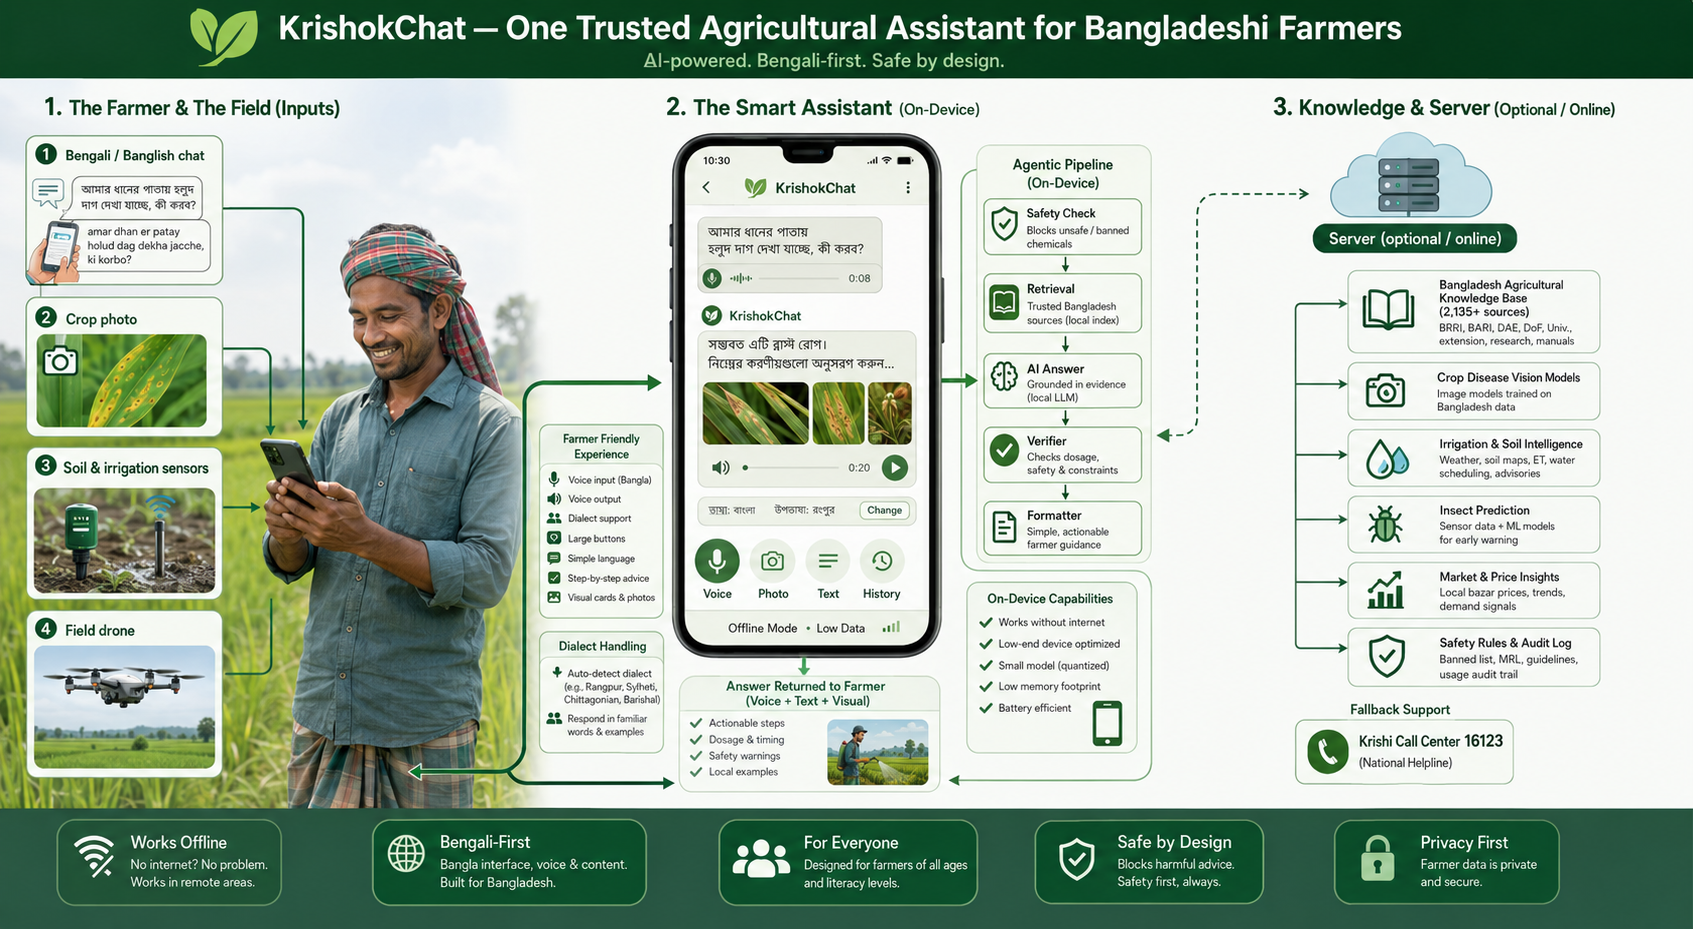
\includegraphics[width=0.96\textwidth]{teaser_diagram.png}
  \caption{KrishokChat at a glance: a farmer's chat, crop photo, soil and irrigation sensors, and field drone feed a single on-device assistant whose safety, retrieval, generation, and verification steps draw on a grounded Bangladesh knowledge base, with the online server optional.}
  \label{fig:teaser}
\end{figure*}

\section{How the System Answers}

KrishokChat is a modular platform that joins language, retrieval, computer vision, and field intelligence behind one simple chat surface. The farmer-facing web app is built with Next.js, Tailwind, and shadcn/ui; the backend is a single Python FastAPI service. Nothing exotic runs in production, which is deliberate: the intelligence lives in the knowledge and the safety design, not in a fragile stack.

\subsection{Grounded Bengali advice, not open guessing}

A quantized Gemma language model is served locally through llama.cpp, so the core assistant does not depend on a paid frontier API to function. Every farmer question is first routed through a safety layer, then matched against a precomputed knowledge base of \stat{2{,}135}{curated knowledge nodes} drawn from Bangladeshi institutional sources. Retrieval uses BM25 today, with hybrid BM25 and dense vector retrieval available for extended configurations. The answer is composed from the retrieved evidence, so the farmer is reading guidance that traces back to a real source passage rather than the model's general memory. The dataset and advisory design behind this work are documented in our public research (\href{https://arxiv.org/abs/2606.29243}{arxiv.org/abs/2606.29243}), and the provenance-traceable retrieval architecture in a companion paper (\href{https://arxiv.org/abs/2608.14886}{arxiv.org/abs/2608.14886}).

\subsection{Safety that runs before the answer, not after}

This is the part that matters most for a food-and-chemical domain. Restricted or banned agrochemical requests are caught before retrieval even begins, checked against a registry of chemicals not approved for use in Bangladesh. Numeric dosage and treatment claims are normalized across Bengali and English number expressions and then verified against the supporting source passage before the answer is released to the farmer. If a self-harm or poisoning risk is detected, the system does not attempt a normal answer; it responds calmly and points to the government's national agricultural helpline, the Krishi Call Center at \stat{16123}{}. Every request and every verification result is written to a local audit record, so the system's safety behavior is measurable rather than assumed.

\subsection{Seeing the field}

For diagnosis, an image pipeline first identifies which crop is in the photo and then hands it to a crop-specific disease model, which is more reliable than one model trying to know every crop at once. Soil and field images feed machine-learning models that support irrigation decisions and flag conditions linked to waterlogging or drought stress. A separate field-intelligence module brings in low-cost sensors and machine learning to monitor and predict insect activity, giving farmers earlier, field-specific alerts instead of reacting after the damage is done. These modules plug into the same advisory surface, so the farmer experiences one assistant, not five disconnected tools.

\section{Why It Holds Up}

We do not ask anyone to take reliability on faith. The system carries a standing engineering baseline of \stat{410}{automated tests passing, 7 skipped, 0 failing}, and a golden replay set of \stat{50}{fixed scenarios} that must reproduce identical, invariant-checked behavior on every change. The safety behavior is backed by a purpose-built dataset of \stat{20{,}112}{safety records} spanning refusal and safe-requery cases across 12 risk categories, six Bengali dialect variants, and dozens of crops, built on a 110-word real dialect map so the assistant understands how farmers actually speak rather than textbook Bengali.

\begin{center}
\begin{tabular}{@{}>{\raggedright\arraybackslash}p{3.3cm} >{\raggedright\arraybackslash}p{4.0cm}@{}}
\arrayrulecolor{brandgreen}\toprule
\textbf{What we tested} & \textbf{Result} \\
\midrule
Automated test suite & 410 passed, 0 failed \\
Golden replay set & 50 / 50 reproduced \\
Safety dataset scale & 20,112 records \\
Risk categories & 12 \\
Dialect coverage & 6 variants, 110-word map \\
Knowledge nodes & 2,135, source-traced \\
Banned-chemical registry & Bangladesh-specific \\
\arrayrulecolor{brandgreen}\bottomrule
\end{tabular}
\end{center}

\section{Prototype and Maturity Level}

KrishokChat is a functional working prototype today, not a concept on paper. The end-to-end path a farmer would use is already running: a photo goes in, the crop and its disease come back, and trusted guidance follows in the same screen.

The disease diagnosis works the way a farmer needs it to. For the crops that matter most in Bangladesh, the image pipeline first recognizes which crop is in the photo and then routes it to a crop-specific disease model, which reaches high accuracy because each model only has to be expert in one crop instead of guessing across all of them. The moment a disease is identified, the system does not stop at a label. It pulls the matching treatment guidance straight from the grounded knowledge base built from government documents and agricultural manuals, so the farmer sees what the problem is and what to do about it, tied to a real source, in one step.

The chatbot works the same practical way. Farmers do not type clean textbook Bengali; they type in dialect, in Banglish, and often ask something vague. The system reads the messy question, classifies what the farmer actually intends behind the wording, and converts that intent into a structured request it can act on, so instead of a loose guess the farmer gets an answer aimed at exactly what they asked, whether that is a disease, a dose, a timing question, or why a crop is failing. The safety layer runs first on every question, catching unsafe or banned-chemical requests before any answer is formed, and every dose is checked against its source before the farmer sees it.

Around this core, the working pieces already include soil and irrigation image analysis, the field-intelligence module for insect monitoring and prediction from low-cost sensors, and the drone-assisted field view, each feeding the same single assistant. The whole system sits on a tested baseline of 410 automated tests passing with a 50-scenario replay set that must reproduce identical behavior on every change, which is what separates a maintainable pilot from a fragile demo. A small number of refinements, the fully offline on-device path and wider crop coverage, are in active development and land within days, before the fair. The committee will see a system that already answers real farmer questions correctly, safely, and with its sources shown, not a slideshow.

\section{How We Compare}

A pesticide dealer has a conflict of interest, a Facebook group has no accountability, and a general chatbot has no Bangladeshi grounding and no safety gate on chemical doses. The table below is the honest comparison a farmer would care about.

\begin{center}
\small
\begin{tabular}{@{}>{\raggedright\arraybackslash}p{2.5cm} c c c@{}}
\arrayrulecolor{brandgreen}\toprule
 & \textbf{Krishok} & \textbf{General} & \textbf{Dealer /} \\
 & \textbf{Chat} & \textbf{chatbot} & \textbf{group} \\
\midrule
Bengali / Banglish native & Yes & Partial & Yes \\
BD-grounded sources & Yes & No & Varies \\
Dose safety check & Yes & No & No \\
Blocks banned chemicals & Yes & No & No \\
Photo diagnosis & Yes & Limited & No \\
Works offline / on device & Designed for & No & n/a \\
Traceable to a source & Yes & No & No \\
\arrayrulecolor{brandgreen}\bottomrule
\end{tabular}
\end{center}

\section{Built to Run Where Farmers Are}

A key design choice is to reduce dependence on large online AI models. The knowledge, the safety rules, and the task-specific vision models are kept separate from the heavy language component, which means the parts that matter most for a farmer, correct doses and safe refusals, can run cheaply and even on device in areas with weak connectivity. Our architecture roadmap formalizes this as a resolution ladder: the most common and highest-risk questions, such as a registered dose for a known crop and disease, are answered from a structured, source-cited table in milliseconds with zero calls to a large model, and the language model is used only to phrase, disambiguate, or handle genuinely novel questions. This is what makes the economics work at farmer scale, and it is being implemented ahead of the fair.

\section{Practical Impact}

Bangladesh has roughly sixteen million farm households, and most decisions about disease and chemicals are made with no expert in reach. KrishokChat puts a calm, source-backed second opinion in the farmer's own language into a phone that is already in his pocket. The direct impact is fewer wrong sprays, less wasted money on the wrong chemical, safer food and water from avoided overdoses, and earlier action on disease and pests before a field is lost. Because the assistant refuses honestly when a question falls outside what it can support, and redirects to the national helpline, it strengthens the existing public extension system instead of competing with it.

\section{Commercialization Potential}

The path to a sustainable product is realistic and layered. The core advisory stays free for farmers, which keeps trust and reach high, while revenue comes from tiers around it: a low-cost premium plan for input dealers, agri-retailers, and cooperatives who need multi-farmer dashboards and record keeping; institutional licensing to NGOs, seed and fertilizer companies, and government extension programs that want a branded, auditable advisory channel; and value-added modules for irrigation, insect prediction, and field monitoring sold to larger farms and agri-enterprises. Because the system is edge-oriented and does not require a frontier API to answer common questions, per-farmer serving cost stays low, which is exactly what allows a free tier to scale without burning capital. The safety audit trail also makes the system defensible for any partner who must show responsible advice, which is a genuine differentiator over generic chatbots.

\section{Contribution to Sustainable Development}

KrishokChat maps directly onto national and global development goals. It supports Zero Hunger by protecting yields and reducing crop loss from mismanaged disease. It supports Responsible Consumption and Production, and clean water, by actively blocking unsafe and banned chemical use and checking every dose. It supports Decent Work and reduced inequality by giving smallholders, including those with low literacy who rely on voice and Banglish, access to the same quality of agronomic guidance that was previously available only to well-connected commercial farms. And by being designed for low-resource, on-device operation, it extends this reach into exactly the rural, low-connectivity areas that are usually left behind.

\section{Where We Are}

Three related research papers document the dataset, the safety-critical advisory design, and the provenance-traceable retrieval architecture, with further system and evaluation work in progress. The application itself is running, tested against a fixed baseline, and backed by a purpose-built safety dataset. The next steps, already planned and underway for the fair, harden the offline and on-device path, extend crop and disease coverage, and add real weather-driven alerting. KrishokChat is not a demo looking for a problem. It is a working answer to a problem farmers face every season, built to be trusted, affordable, and ready to scale.

\end{multicols}

\end{document}
